\documentclass{article}

\usepackage[submission]{colm2026_conference}
\usepackage{microtype}
\usepackage{hyperref}
\usepackage{url}
\usepackage{booktabs}
\usepackage{amsmath}
\usepackage{array}
\usepackage{graphicx}
\usepackage{xcolor}
\usepackage{lineno}

\definecolor{darkblue}{rgb}{0, 0, 0.5}
\hypersetup{colorlinks=true, citecolor=darkblue, linkcolor=darkblue, urlcolor=darkblue}

\title{Beyond PII Removal: Risk-Budgeted Generalization for LLM-Ready Sensitive Text}
\author{Anonymous Authors}

\begin{document}

\ifcolmsubmission
\linenumbers
\fi

\maketitle

\begin{abstract}
Sensitive text corpora are valuable for retrieval, evaluation, and
post-training adaptation of foundation-model systems, but common
de-identification pipelines still center on direct personally identifying
information (PII): names, emails, phone numbers, addresses, and account
numbers. This is necessary but incomplete. A record with no explicit name can
still reveal sensitive attributes through quasi-identifiers such as exact
dates, fine-grained locations, rare occupations, institutions, family
relations, clinical or legal events, citizenship cues, and combinations of
ordinary facts. We introduce Risk-Budgeted Quasi-Identifier Generalization
(RB-QIG), a lightweight transformation policy that treats de-identification as
a privacy--utility allocation problem: given candidate quasi-identifiers,
which facts should be kept, generalized, or redacted under a document-level
risk budget? RB-QIG uses transparent risk and utility scores, span-level
generalization ladders, and a greedy audit log rather than model training or
unconstrained rewriting. Across synthetic, RAT-Bench, and TAB pilots, the
central pattern is consistent: direct PII redaction and naive LLM sanitization
leave substantial residual inference risk, while explicit quasi-identifier
transformation sharply reduces measured leakage. The strongest utility result
is controlled: on synthetic records, RB-QIG preserves far more utility facts
than blanket quasi-identifier redaction at a nonzero but much lower leakage
level. Public utility is more mixed, and stronger GPT-5.5 attackers recover
more from all methods, so RB-QIG should not be read as an anonymization
guarantee. Instead, the result is a practical argument for evaluating what
capable models can still infer, not only which explicit PII spans were
removed.
\end{abstract}

\section{Introduction}

Sensitive text is one of the most tempting and most difficult data sources for
foundation-model systems. Clinical notes, legal opinions, financial
communications, student-support records, workplace logs, and user-assistant
conversations contain the domain knowledge that makes retrieval and adaptation
useful. They also contain facts that can identify, profile, or expose people.
Responsible data enablement therefore often starts with a familiar
transformation step: remove names, emails, phone numbers, addresses, and other
direct identifiers.

This paper asks what remains after that step. A sentence such as ``a
34-year-old oncology infusion pharmacist at a small startup in Asheville
called about a brother's rare condition after an April 2025 surgery'' can be
name-free and still highly revealing. The risk is not a single missed token; it
is the combination of age, job, location, relationship, date, and rare event.
Classical privacy work formalized this linkage problem through
quasi-identifiers and group-based anonymization
\cite{sweeney2002kanonymity,machanavajjhala2007ldiversity,li2007tcloseness,fung2010survey,narayanan2008netflix}.
Regulatory and policy guidance also recognizes that identifiability can arise
directly or indirectly, and that residual information may be identifying in
combination with other available information
\cite{gdpr2016,hhsHipaaDeidentification,nist800122}.

Large language models make this residual-risk problem more visible. They can
combine paraphrases, world knowledge, and conversational cues to infer private
attributes that are not explicitly stated \cite{staab2023beyond}. Recent work
on semantic privacy and implicit inference argues that users and systems often
underestimate what can be inferred from ordinary text
\cite{ma2025semantic,wang2025beyondpii}. Text anonymization benchmarks such as
TAB and RAT-Bench likewise move beyond direct PII spans toward residual
re-identification risk and utility preservation
\cite{pilan2022tab,krco2026ratbench}.

\begin{figure}[t]
\centering
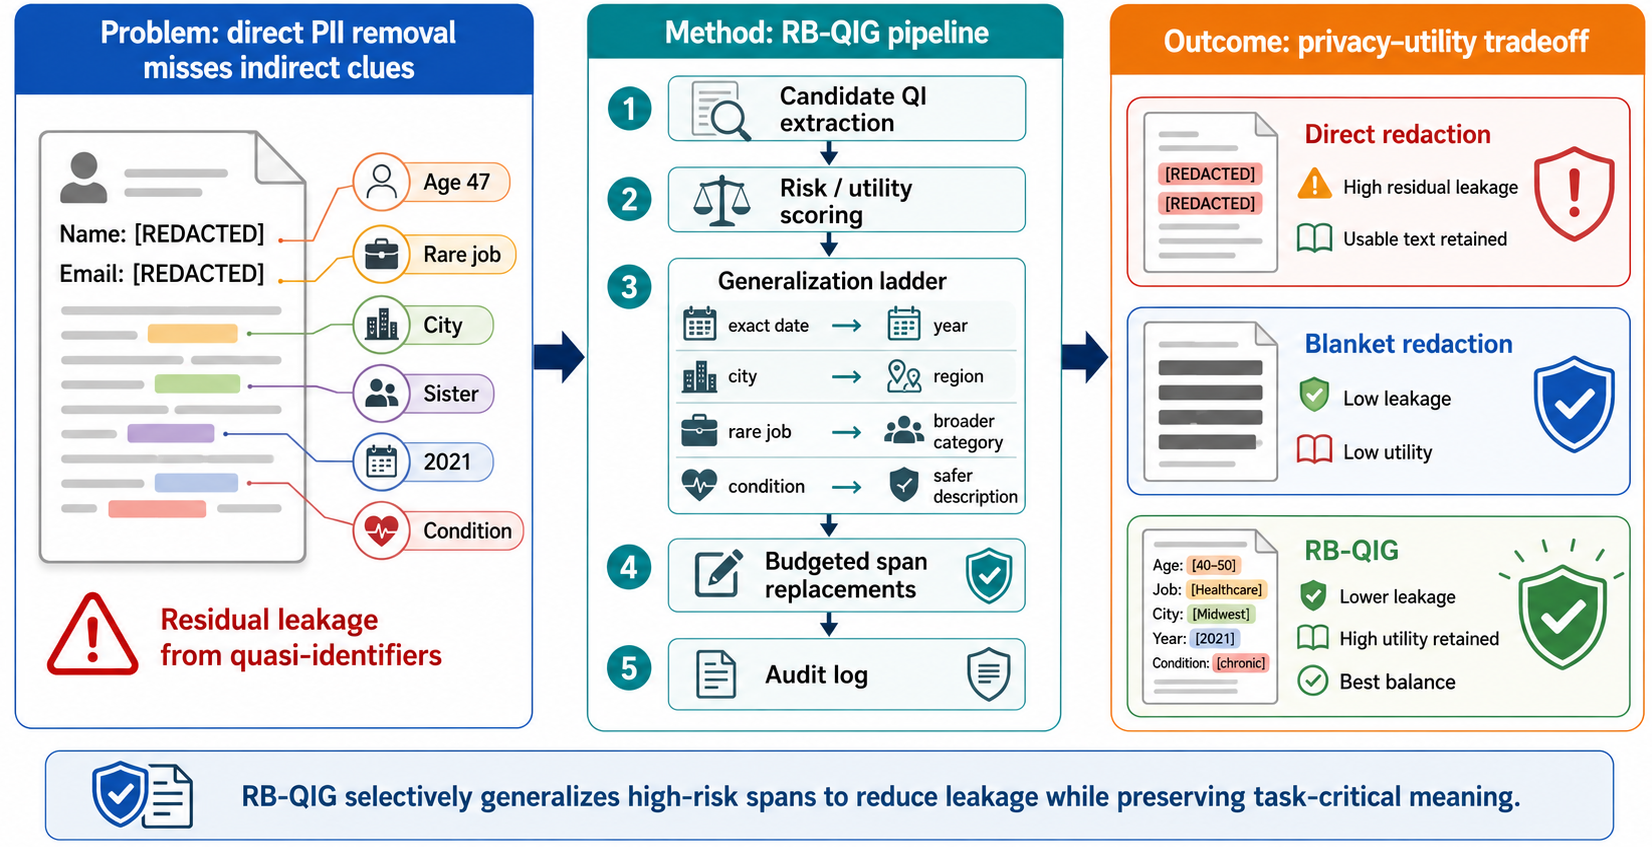
\includegraphics[width=\linewidth]{figure/figure_1.png}
\caption{Conceptual overview of RB-QIG. Direct PII removal can leave indirect
quasi-identifier clues; RB-QIG extracts candidate QIs, scores privacy risk and
utility, and applies budgeted generalization so high-risk spans are coarsened
rather than always left intact or blanket-redacted.}
\label{fig:overview}
\end{figure}

The practical design question is therefore not ``did a recognizer remove every
PII span?'' but ``what can an attacker still infer, and how much useful meaning
survives the transformation?'' Direct PII removal is utility-preserving but
leaky. Blanket quasi-identifier redaction is safer but often destroys the
semantics that make the data useful. We study the middle ground: targeted
generalization. For example, ``oncology infusion pharmacist in Asheville'' can
become ``clinical pharmacy professional in a city in the southeastern U.S.''
rather than either being left intact or replaced with opaque placeholders.

We introduce Risk-Budgeted Quasi-Identifier Generalization (RB-QIG), a small
auditable policy layer for sensitive text. RB-QIG does not train a model and
does not rewrite whole documents. It assumes candidate quasi-identifier spans
from an oracle, benchmark-aware extractor, or blind extractor; assigns each
candidate a privacy-risk score and a utility-importance score; and applies the
least destructive replacement needed to meet a document-level risk budget. Each
edit is logged, making the policy inspectable by data owners.

Our contributions are:
\begin{itemize}
\item a taxonomy and transformation view of quasi-identifiers for LLM-ready
sensitive text;
\item a risk-budgeted span-generalization algorithm that exposes a tunable
privacy--utility frontier without fine-tuning;
\item an evaluation protocol combining deterministic leakage metrics, LLM
attackers, stronger-attacker checks, and utility diagnostics; and
\item an empirical analysis showing that direct redaction fails because
sensitive attributes remain inferable from relational, lexical, and contextual
cues.
\end{itemize}


\section{Background}

\paragraph{Direct identifiers, quasi-identifiers, and sensitive attributes.}
We use \emph{direct identifier} for a span that directly identifies a person or
account: a name, email, phone number, address, account ID, or equivalent. We
use \emph{quasi-identifier} (QI) for a fact that may not identify a person
alone but becomes identifying or sensitive in combination with other facts.
Examples include ages, dates, locations, rare occupations, schools, employers,
family relations, medical events, legal events, citizenship status, and
cultural cues. We use \emph{sensitive attribute} for the attribute an attacker
tries to recover, such as sex, race/ethnicity, citizenship, marital status,
education, employment, or a domain-specific clinical/legal fact.

\paragraph{Why text is harder than tables.}
Classical anonymization methods were developed largely for structured records,
where each row has known columns and generalization can be specified over
attribute hierarchies \cite{sweeney2002kanonymity,machanavajjhala2007ldiversity,li2007tcloseness}.
Text does not offer that clean schema. The same cue may appear as a named
entity, a narrative phrase, a family relation, a quoted statement, or a
placeholder created by a previous sanitizer. Recent medical and general text
work has therefore emphasized indirect identifiers and LLM-based inference
risks \cite{baroud2025beyond,jiang2026paradox,staab2024advanced,yang2024rupta}.

\paragraph{Threat model.}
The attacker receives transformed text. In our LLM-attacker evaluations, the
attacker is asked to infer benchmark attributes and return structured guesses
with short evidence. We score exact recovery, coarse recovery, record
compromise, and risk-weighted leakage. The attacker is not asked to identify
real people, and all experiments use synthetic or public benchmark data. This
is not a complete model of arbitrary external databases or determined human
investigators. It is a reproducible stress test for whether a transformation
leaves sensitive attributes inferable from the transformed text itself.

\paragraph{Three evaluation settings.}
We separate transformation quality from extraction realism. In the
\emph{controlled} setting, oracle quasi-identifier spans are known from
synthetic profiles. In the \emph{target-aware public} setting, benchmark target
attributes are used to find value-revealing spans, isolating how well
transformations work when the sensitive attributes of interest are known. In
the \emph{blind public} setting, the extractor does not see target attributes
at extraction time and is scored afterward. The blind setting is closest to
deployment and is the main source of our limitations.

\section{Risk-Budgeted Quasi-Identifier Generalization}

\subsection{Conceptual Design}

RB-QIG treats de-identification as a budgeted editing problem. For each
candidate quasi-identifier $q_i$, the system stores: (1) its text span; (2) a
type such as \textsc{age}, \textsc{location}, \textsc{occupation}, or
\textsc{family}; (3) a privacy-risk score; (4) a utility-importance score; and
(5) a short ladder of possible replacements. Table~\ref{tab:taxonomy} shows the
main QI types.

\begin{table}[t]
\centering
\small
\caption{Examples of quasi-identifier categories and generalization ladders.
The method uses span replacements rather than unconstrained rewriting, so every
edit can be audited.}
\label{tab:taxonomy}
\begin{tabular}{lll}
\toprule
Category & Precise cue & Generalized cue \\
\midrule
Date/age & April 17, 2025; 34 & month/year; 30s \\
Location & Asheville, NC & city in the southeastern U.S. \\
Occupation & oncology infusion pharmacist & clinical pharmacy professional \\
Institution & named school or employer & university; healthcare company \\
Medical/legal event & rare condition or case event & broader condition/event type \\
Family relation & younger brother under guardianship & dependent family member \\
Demographic cue & citizenship or heritage phrase & broader demographic phrase \\
Narrative cue & unusual life event & coarse role-preserving description \\
\bottomrule
\end{tabular}
\end{table}

The important distinction is between \emph{redaction} and
\emph{generalization}. Redaction replaces a value with a placeholder such as
\texttt{[LOCATION]}. Generalization keeps a coarser version of the useful
semantics, such as ``city in the southeastern U.S.''. RB-QIG's hypothesis is
that many sensitive-data uses do not require exact quasi-identifiers; they
require enough contextual information for the downstream task.

\subsection{Scoring and Budgeted Editing}

Each candidate $q_i$ receives a risk score $r_i \in [0,5]$ and utility score
$u_i \in [0,5]$. Risk reflects specificity, rarity, sensitivity, and
linkability. Utility reflects whether the fact is useful for the benign task.
For instance, a diagnosis family may be useful in a medical-support note,
whereas the exact surgery date may not be.

The document risk score is
\[
R(x) = \sum_i r_i + 0.5 \binom{|\{i:r_i \geq 3\}|}{2},
\]
where the second term is a simple combination-risk penalty: multiple
high-specificity cues are more dangerous together than separately. Each
candidate replacement has an estimated risk drop and utility cost. RB-QIG
greedily applies the next replacement with the best risk-drop-per-utility-loss
ratio until the risk budget is met or no replacement remains. The output is
the transformed text plus an edit log.

This scoring rule is deliberately simple. It is not a universal privacy
estimate. Its role is to make a data owner's policy explicit: which facts are
risky, which facts are useful, how much residual risk is tolerated, and which
semantic abstractions are acceptable.

\subsection{Baselines}

We compare RB-QIG against conceptual and practical baselines:
\emph{none} (unchanged text), \emph{direct redaction} (direct identifiers only),
\emph{naive LLM direct} (an LLM instructed to remove identifying information
while preserving meaning), \emph{blanket QI redaction} (all QIs become typed
placeholders), and a \emph{Presidio-style pattern baseline}. The pattern
baseline is a practical lower-bound diagnostic, not a full production Presidio
deployment.

\section{Experiments}

\paragraph{Datasets.}
The controlled benchmark contains 100 synthetic records across medical, legal,
financial, workplace, and education-support domains. Each record has direct
identifiers, QIs, target attributes, a task label, and utility facts. The
public text benchmark is a 100-record English difficulty-1 RAT-Bench pilot
\cite{krco2026ratbench}. We also run a 30-document TAB ECHR legal screen
\cite{pilan2022tab}. These public datasets are used as stress tests rather
than claims of benchmark saturation.

\paragraph{Evaluators.}
Deterministic evaluators score explicit attribute leakage, QI specificity, and
token change. LLM attackers score whether target attributes can be recovered
from transformed text. LLM utility judges score label preservation,
fact preservation, and semantic utility without rewarding preserved direct
identifiers. Additional bounded checks use GPT-5.5 as a stronger attacker and
a mini-model agreement screen to test model dependence. All API calls use
synthetic or public benchmark records.

\paragraph{Metrics.}
We report risk-weighted leakage as the primary privacy metric. Utility is
measured with utility-fact preservation in the controlled setting, semantic
utility in LLM-judge settings, and annotation-derived QI specificity as a
narrow no-API proxy for whether typed/generalized semantics survive. To keep
the main paper readable, the results section emphasizes headline patterns; the
appendix contains the detailed numeric tables.

\begin{figure}[t]
\centering
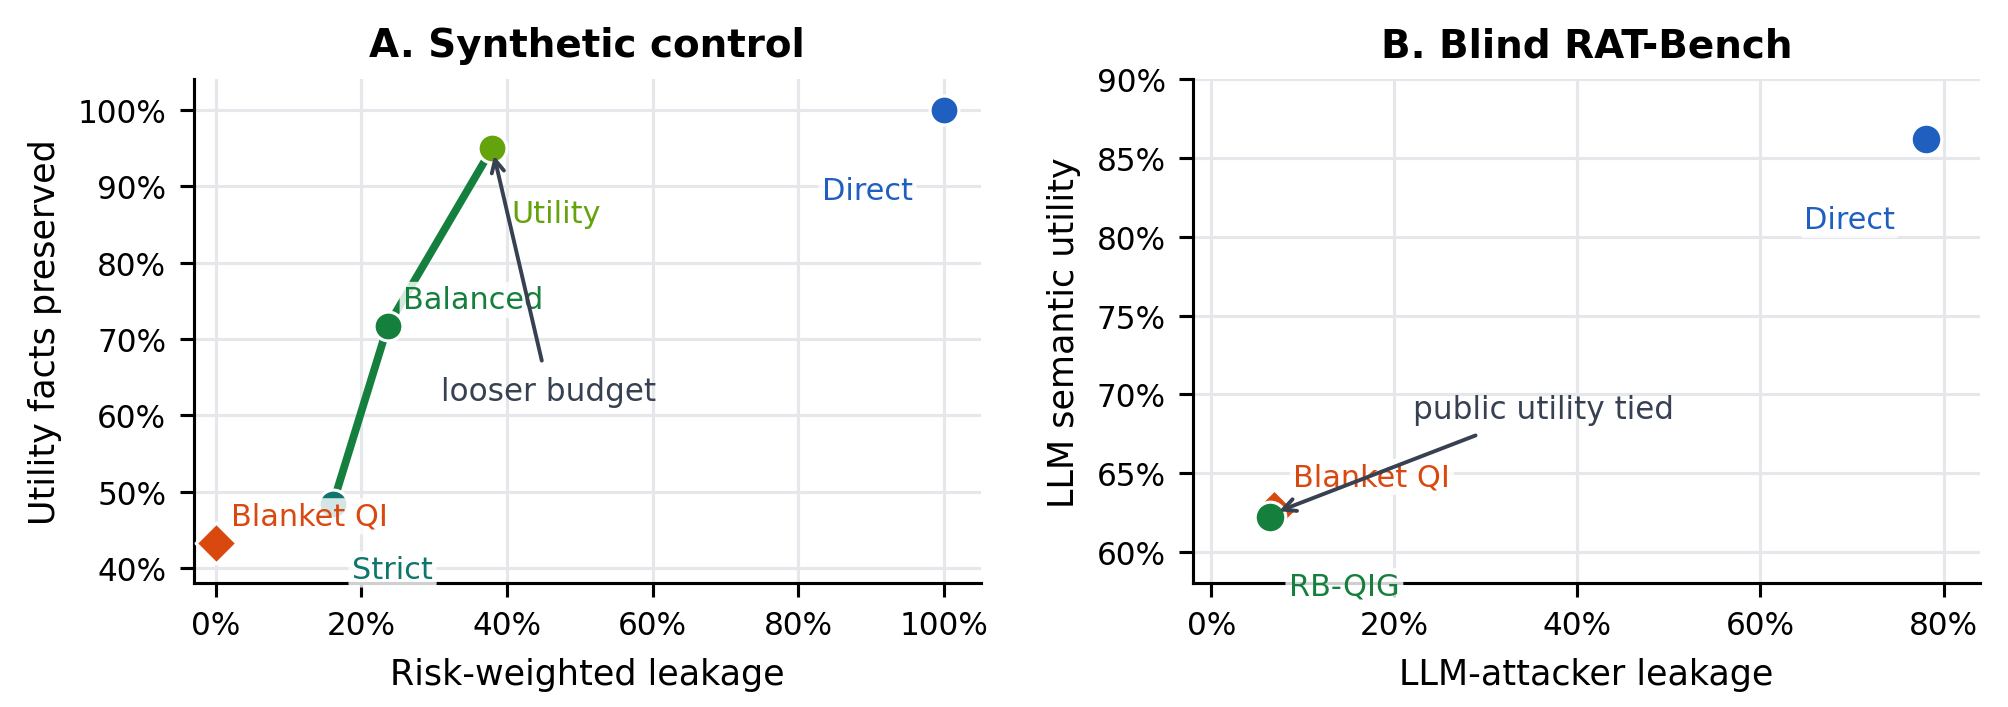
\includegraphics[width=\linewidth]{figure/figure_2.png}
\caption{Privacy--utility frontier. Panel A uses deterministic synthetic
metrics: direct redaction preserves utility facts but leaks QIs, blanket QI
redaction removes measured leakage with lower utility, and RB-QIG budgets
trace an intermediate frontier. Panel B uses blind RAT-Bench LLM attacker and
utility judges; RB-QIG and blanket redaction are close on public utility.}
\label{fig:frontier}
\end{figure}

\section{Results}

\begin{table}[t]
\centering
\small
\caption{Main results.}
\label{tab:headline}
\begingroup
\renewcommand{\arraystretch}{1.5}
\begin{tabular}{p{0.25\linewidth}p{0.34\linewidth}p{0.32\linewidth}}
\toprule
Question & Main observation & Interpretation \\
\midrule
Does direct PII redaction suffice? &
No. RAT-Bench direct redaction leaves high LLM-attacker leakage. &
Sensitive attributes remain inferable from QIs and context. \\
Can RB-QIG reduce residual risk? &
Yes. RB-QIG sharply lowers leakage relative to direct and naive LLM redaction. &
Explicit QI transformation is necessary for LLM-ready text. \\
Is RB-QIG more private than blanket QI redaction? &
No clear evidence. They are usually tied under LLM attackers. &
The value of RB-QIG is utility-aware transformation, not privacy dominance. \\
Where is the utility win? &
Strong in synthetic utility facts; weak or tied in public utility judges. &
Utility-preserving blind rewriting remains the main open problem. \\
Do stronger attackers change the conclusion? &
GPT-5.5 increases absolute leakage, but the method ordering remains. &
Residual risk is real; robust evaluation needs strong attackers. \\
\bottomrule
\end{tabular}
\endgroup
\end{table}

\paragraph{Result 1: direct PII redaction is the wrong endpoint.}
Across the RAT-Bench pilots, removing direct identifiers leaves substantial
recoverable information. The target-aware LLM attacker still recovers many
attributes after direct redaction, and the blind public setting shows the same
qualitative failure. A naive LLM sanitizer improves over direct redaction but
does not close the gap. The takeaway is simple: for LLM-ready sensitive text,
PII removal is a first pass, not a complete transformation.

\paragraph{Result 2: RB-QIG gives a controlled middle ground.}
The cleanest privacy--utility result is the synthetic control
(Figure~\ref{fig:frontier}). Direct redaction preserves the utility facts but
leaves QI leakage. Blanket QI redaction removes measured leakage but discards
much of the useful semantics. RB-QIG balanced sits between these extremes:
it greatly reduces leakage while preserving substantially more utility facts
than blanket redaction. This is the paper's strongest positive utility claim,
and it should stay scoped to the controlled setting.

\paragraph{Result 3: public utility is the caveat, not the headline.}
On blind public RAT-Bench, RB-QIG and blanket redaction are similar under the
LLM utility judge. Additional placeholder, fluent-rewrite, and
attribute-level fluent diagnostics did not convert this into a clear public
utility win. The text-quality audit suggests that surface fluency alone is not
the missing ingredient: cleaner phrase-level rewrites can still remove the
facts needed for hidden-label utility. This points toward a more difficult
future direction: task-aware generalization rather than prettier replacement
phrases.

\paragraph{Result 4: stronger attackers raise leakage but preserve the
ordering.}
A bounded GPT-5.5 attacker check is harsher than the low-cost attacker:
absolute leakage rises for all privacy-preserving methods. However, direct
redaction remains much leakier than RB-QIG or blanket QI redaction, and a
mini-model agreement check gives the same qualitative ordering. This supports
the use of strong attackers as robustness tests, while reinforcing that RB-QIG
is not an anonymization guarantee.

\begin{figure}[t]
\centering
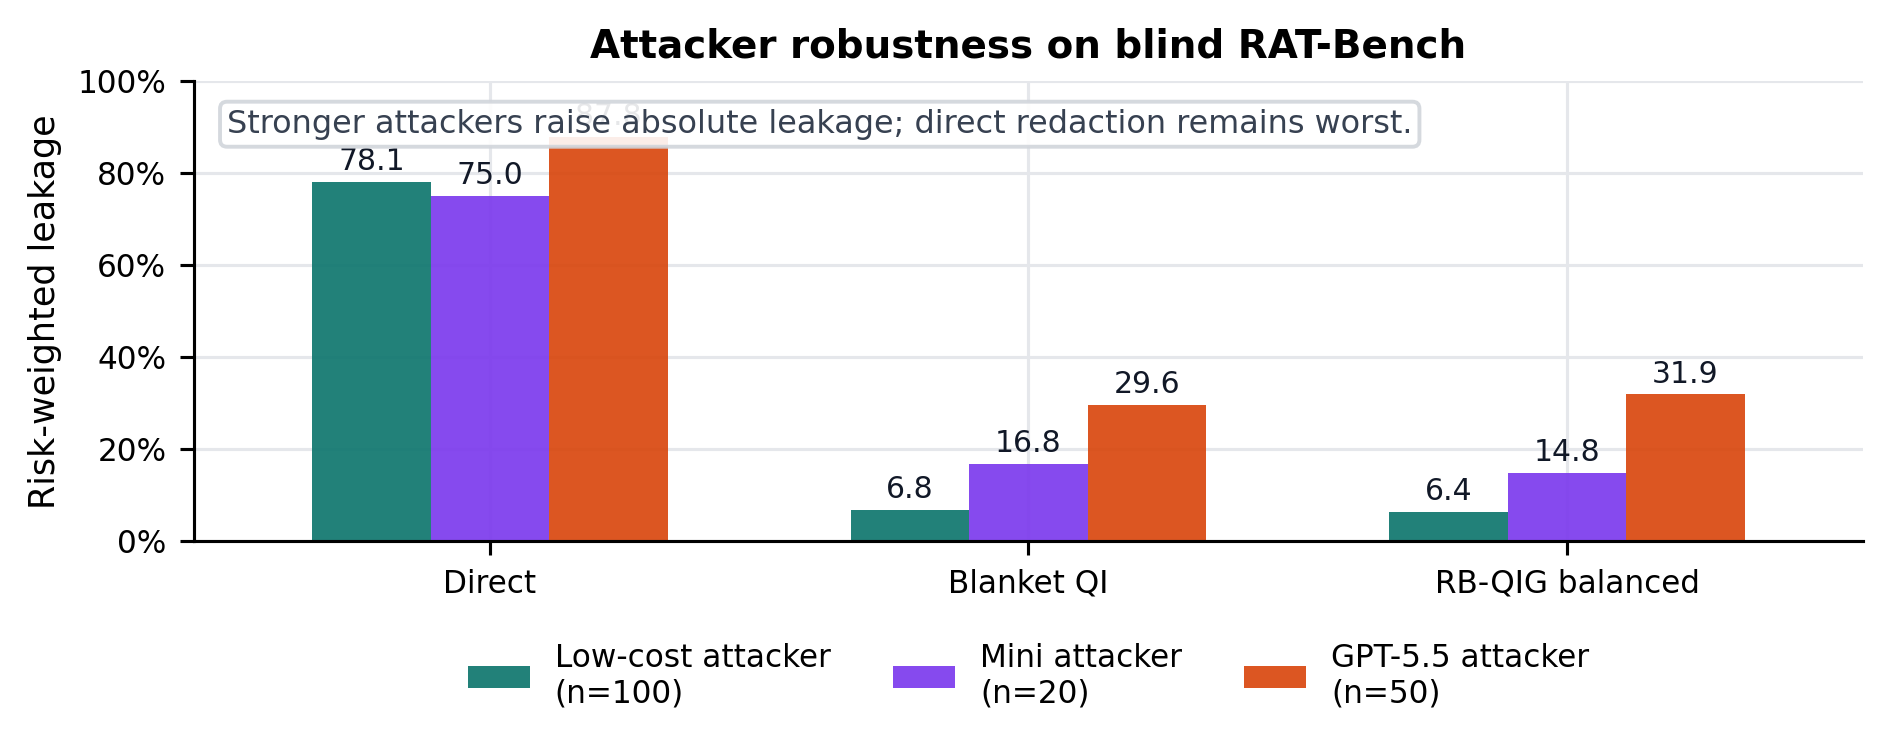
\includegraphics[width=\linewidth]{figure/figure_3.png}
\caption{Attacker robustness on blind RAT-Bench. Bars are for
low-cost, mini, and GPT-5.5 attackers with sample sizes shown in the legend.
Stronger attackers raise absolute leakage, but direct redaction remains much
leakier than RB-QIG or blanket QI redaction.}
\label{fig:robustness}
\end{figure}

\paragraph{Result 5: the risk budget behaves like a real control knob.}
Budget-frontier diagnostics show the expected behavior on blind RAT-Bench and
TAB: stricter budgets reduce leakage but also reduce annotation-derived
specificity, while looser budgets preserve more typed or generalized QI
semantics at higher residual risk. This is important because RB-QIG is meant to
be a policy interface. Different data owners may choose different budgets
depending on the recipient, task, and review process.

\begin{figure}[t]
\centering
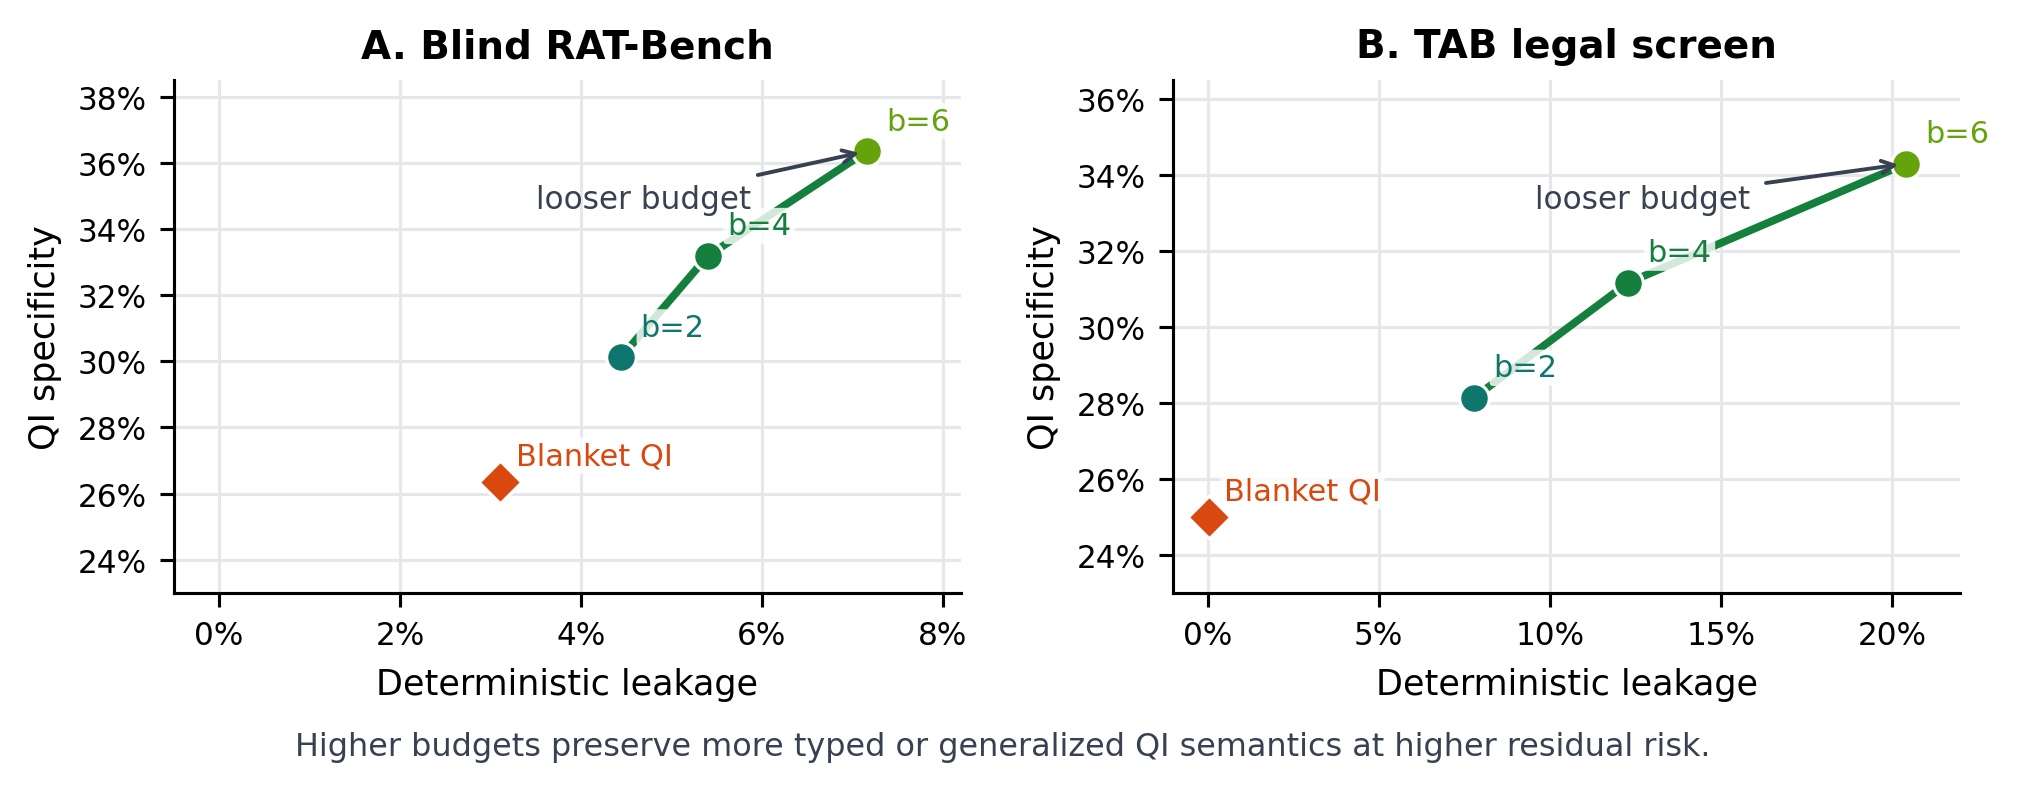
\includegraphics[width=\linewidth]{figure/figure_4.png}
\caption{Budget frontier and domain transfer. Deterministic budget sweeps on
blind RAT-Bench and TAB show that looser RB-QIG budgets preserve more
annotation-derived QI specificity at higher leakage, while blanket QI
redaction stays low-specificity.}
\label{fig:budget}
\end{figure}

\paragraph{Cross-domain and practical-baseline diagnostics.}
The TAB legal screen supports the residual-risk story in a second domain:
direct redaction leaves many legal and narrative cues, while RB-QIG reduces
deterministic leakage. However, the bounded legal-task utility screen is tied
or slightly worse than blanket redaction, so TAB should be presented as
cross-domain privacy evidence rather than a utility win. The Presidio-style
pattern baseline provides a practical lower-bound diagnostic: pattern-only
redaction misses many domain-specific identifiers, especially legal names and
case identifiers.

\paragraph{Failure modes.}
Residual leaks usually come from relational or lexical cues rather than missed
obvious spans: bereavement language can imply marital status, gendered family
roles can imply sex, cultural references can imply race or ethnicity,
citizenship phrasing can reveal immigration status, and institutions can reveal
education or employment. These failures explain why span recall alone is an
incomplete privacy metric.

\begin{table}[t]
\centering
\begingroup
\setlength{\tabcolsep}{2pt}
\renewcommand{\arraystretch}{1.5}
\footnotesize
\caption{Representative residual failure categories.}
\label{tab:failure-categories}
\begin{tabular}{p{0.17\linewidth}p{0.22\linewidth}p{0.30\linewidth}p{0.21\linewidth}}
\toprule
Failure type & Example cue & Why span removal misses it & Possible fix \\
\midrule
Relation cue & bereavement or family-status phrase & sensitive status is inferred from a relation, not named directly & relation-aware rewrite \\
Gender cue & pronouns or gendered family roles & sex can be inferred after direct identifiers are removed & neutralization pass \\
Cultural cue & heritage, tradition, or language mention & race or ethnicity may be inferred from ordinary context & coarser cultural phrase \\
Institution cue & school, employer, or service branch & education or employment is exposed by a named institution & institution ladder \\
Placeholder cue & typed demographic placeholder in context & the placeholder itself can reveal the attribute class & neutral placeholders \\
\bottomrule
\end{tabular}
\endgroup
\end{table}

\section{Limitations and Ethics}

The strongest utility result is synthetic and controlled;
public utility preservation remains mixed. The blind extractor and deterministic backstop improve
coverage, yet blind QI extraction and task-aware rewriting remain open
problems. LLM attackers and utility judges are model-dependent and may under- or over-estimate real adversaries or human
utility needs. All experiments use synthetic or public benchmark data. We do
not attempt to identify real people or infer private attributes about
individuals.

\section{Conclusion}

Direct PII removal is an incomplete transformation for LLM-ready sensitive
text. RB-QIG reframes de-identification as a risk-budgeted generalization
problem: identify quasi-identifiers, score their privacy and utility roles, and
choose the least destructive replacements that meet a risk budget. The current
evidence supports a clear message. Direct redaction and naive LLM sanitization
leave substantial residual inference risk; explicit QI transformation sharply
reduces that risk; controlled utility can be preserved better than blanket
redaction; and blind, task-aware utility preservation remains the main open
problem. Responsible data enablement should therefore evaluate what capable
models can still infer, not only what explicit PII spans were removed.


\bibliographystyle{colm2026_conference}
\bibliography{references}

\end{document}
